\documentclass[a4paper,titlepage]{article}
\usepackage[utf8]{inputenc}
\usepackage{a4wide}
\usepackage[T1]{fontenc}
\usepackage{times}
\usepackage{color}
\usepackage[dvipsnames]{xcolor}
\usepackage{fancyhdr} %% Package to create a header on each page.
\usepackage{lastpage} %% Used for "Page X of Y" in the header.
\usepackage{refcount}
\usepackage{fp}
\newcommand{\pagerefprev}[1]{
	 \FPeval{\result}{clip(\getpagerefnumber{#1}-1)}
	 \result
}

% German
\usepackage[ngerman]{babel}
% English
%\usepackage[english]{babel}

\usepackage[round,authoryear]{natbib}
\usepackage{amsmath,amssymb,amsthm}
\usepackage[hyphens]{url}
\usepackage[colorlinks=true, urlcolor=blue, linkcolor=black ]{hyperref}
\usepackage{graphicx}
\usepackage{wrapfig}
\usepackage{subcaption}
\usepackage{float}
\usepackage[font=small,labelfont=bf]{caption}
\usepackage[title]{appendix}
\usepackage{enumitem}

\usepackage{scrextend}
\deffootnote[1em]{1em}{1em}{\textsuperscript{\makebox[1em][l]{\thefootnotemark}}} %no indent of footnote

%inline code formating
\usepackage{xcolor}
\definecolor{codeColor}{gray}{0.1}
\newcommand{\ilc}[1]{\textcolor{codeColor}{\texttt{#1}}}

\fancyhf{}
%% Left side of header
\lhead{\titleName}
%% Height of header
%\usepackage[top=2.5cm,bottom=2.5cm, left = 2cm, right=2cm]{geometry}
%% Right side of footer
\rhead{Seite \thepage\ von\pagerefprev{appendixPage}}
%% Page style that uses the header
\pagestyle{fancy}

\newcommand{\titleName}{Multi Device Feed}
\renewcommand{\thefigure}{\thesection.\arabic{figure}}

\setlength{\parindent}{0pt}
\usepackage[parfill]{parskip}
\setlength{\parskip}{0.8em}

\begin{document}

% Titelseite
% - - - - - - - - - - - - - - - - - - - - - - - 

\begin{titlepage}
	\begin{tabular}{@{}ll}
		Kurs: &\indent Introduction to Internet and Security (IaS), Frühjahrsemester 2021  \\
		Dozenten: &\indent Prof. Dr. Christian Tschudin  \\
		Datum: &\indent 18. Juli 2021
	\end{tabular}
	\vspace*{1cm}   
	\begin{center}
		\large
		{\color{NavyBlue}{Projekt Report}} \\	
		\vspace*{1cm}   
	        \Huge
	        {\color{NavyBlue}{BACnet: \\ \titleName}}\\
	        \Large
        	\vspace*{1cm}   
	        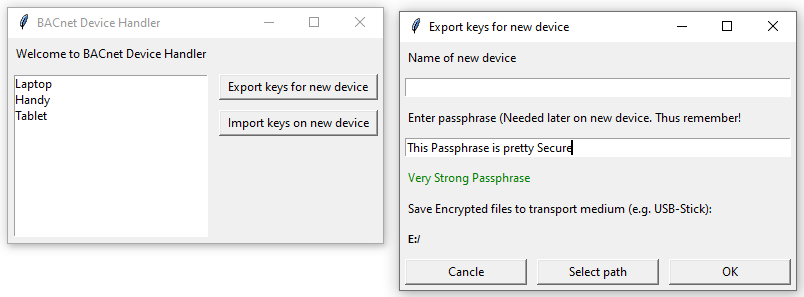
\includegraphics[width=0.75\textwidth]{figures/UI}  
		\vfill
	        \normalsize
		\begin{tabular}{@{}ll}
			Gruppe 10 \\
			Matthias Müller &\indent \href{mailto:matthias01.mueller@stud.unibas.ch}{matthias01.mueller@stud.unibas.ch}  \\
			Patrick Steiner &\indent \href{mailto:pa.steiner@stud.unibas.ch}{pa.steiner@stud.unibas.ch}  \\
			Reto Krummenacher &\indent \href{mailto:reto.krummenacher@unibas.ch}{reto.krummenacher@unibas.ch}
		\end{tabular}
	\end{center}  
\end{titlepage}

% Report
% - - - - - - - - - - - - - - - - - - - - - - - 
\clearpage
\setcounter{page}{1}


\section{Einleitung}

Das BACnet ist eine dezentralisiertes Netzwerk, welche ohne das Internet und dessen gängige Protokolle (IP, TCP) die Kommunikation zwischen Teilnehmern ermöglicht. Die einfachste Art der Informationsübertagung ist die Übergabe von USB-Sticks mit den gewünschten Daten der Applikationen. Jede Applikation erstellt ihre eigenen Feeds mit einem privaten und öffentlichen Schlüssel. Eine Feed kann als erweiterbare aber nicht veränderbare verkettete Liste betrachtet werden. Anhand des öffentlichen Schlüssels sind die einzelnen Feeds unterscheidbar. Ein Nutzer im BACnet wird anhand eines sogenannten Master-Feeds\footnote{Dies basiert auf Arbeiten aus dem Frühjahressemester 2020: \\ \url{https://github.com/cn-uofbasel/BACnet/tree/master/20-fs-ias-lec/groups/14-feedCtrl} \\ (letzter Aufruf 11.07.2021)} eindeutig identifiziert.

Bisher war es einem Teilnehmer im BACnet nicht möglich, die gleiche Applikation von verschiedenen Geräten zu bedienen. Dazu müssen einerseits die Privaten Schlüssel der Feeds geteilt werden, damit der gleiche Benutzer auf einem anderen Gerät die selben Feeds erweitern kann. Damit besteht die Gefahr von Kollisionen. Ein Nutzer schreibt von Gerät A und B gleichzeitig in einen Chat. Das dezentrale BACnet hat keine automatische Synchronisation, sprich die Daten von Gerät A werden nicht sofort auf das Gerät B übertragen. Für den Chatpartner müssen die Einträge von Gerät A und B zusammengefügt werden. Mit der BACnet Prämisse von nicht veränderbaren Feeds ist dies nicht möglich. Eine Lösung sind virtuelle Feeds.

Ziel dieses Begleitprojekts im Rahmen der Vorlesung `Internet and Security' ist das Entwickeln eines Systems virtueller Feeds für das BACnet sowie einer Möglichkeit der Geräteverwaltung für den Benutzer. Der vorliegende Bericht erläutert die erarbeiteten Lösungen und beschreibt die erstellten Python-Module \footnote{Sämtlicher Code findet sich unter: \\ \url{...} \textcolor{red}{link zum code auf GitHub}} konzeptionell. In einem ersten Teil werden die virtuellen Feeds behandelt während die Geräteverwaltung in einem zweiten Teil besprochen wird. Abschluss bildet die kritische Würdigung der Arbeiten. Im Anhang finden sich sämtliche Abbildungen sowie die Liste mit den benützten Python-libraries.


\section{Virtuelle Feeds}


\section{Geräteverwaltung}
Die Hauptaufgaben der Geräteverwaltung ist das verteilen von privaten Feed-Schlüssel auf weitere Geräte eines Nutzers. Die Klassen und Methoden finden sich im Modul `deviceHandler' und stellen einerseits die Funktionalität als auch eine GUI bereit.

\subsection{Funktionalität}
Die gesamte Funktionalität ist in \ilc{uiFunctions.py} implementiert. 

\subsubsection*{Schlüsselverteilung}
Das verteilen von privaten Schlüssel ist unter dem Begriff `Key exchange problem' bekannt. Dies kann mittels Verwendung eines asymmetrischen Schlüsselpaars umgangen werden. Zu sendende Nachrichten werden mit dem öffentlichen Schlüssel des Empfängers verschlüsselt. Nur mit dem privaten Schlüssel des Empfängers ist eine Entschlüsseln möglich. Im vorliegenden Fall ist dies nicht praktikabel, da das Erstellen eines asymmetrischen Schlüsselpaars den Austausch der dazu notwendigen Informationen benötigt. Im dezentralen BACnet erfordert dies ein mehrmaliges hin und her reichen eines USB-Sticks. Aus diesem Grund haben wir uns für eine symmetrischen Verschlüsselungsverfahren mit einem gemeinsamen privaten Schlüssel entschieden. 

Unser Lösungsansatz ist, dass der private Schlüssel gar nicht geteilt, sonder auf jedem Gerät individuell erstellt wird. Dazu verwenden wird den gleichen Algorithmus auf beiden Geräten zusammen mit einem vom Benutzer bereitgestellten Password. Dieses Verfahren ist als `password based key derivation' bekannten und von der IETF\footnote{Internet Engineering Task Force, RFC 8018, Password-Based Cryptography Specification Version 2.1\\ \url{https://datatracker.ietf.org/doc/html/rfc8018\#appendix-A.2} \\ (letzter Aufruf 11.07.2021)} empfohlen. Die Daten, hier die privaten Schlüssel aller Feeds eines Benutzers, werden mit dem passwortbasierten Schlüssel auf Gerät A verschlüsselt und auf einem Transportmedium gespeichert. Nur mit dem Passwort ist das Entschlüsseln auf Gerät B möglich.

Um die Stärke des eingegebenen Passworts zu bewerten, wird dessen Entropie berechnet. Die Entropie wird durch die Länge und die möglichen Anzahl der Zeichen bestimmt.\footnote{Berechnung der Entropy im Detail: \\ \url{https://www.omnicalculator.com/other/password-entropy} \\ (letzer Aufruf 9.7.2021)} Je höher der Wert, desto mehr Möglichkeiten ($2^{Entropie}$) gibt es. Entsprechenden länger dauert ein Brut-Force erraten des Passworts.

\subsubsection*{Geräte hinzufügen und löschen}




\subsection{GUI}
Die graphische Benutzeroberfläche wurde mit \ilc{tkinter} erstellt und ist in \ilc{ui.py} implementiert. Das Hauptfenster ermöglicht dem Benutzer die Funktionalitäten der Geräteverwaltung per Klick auszuführen. Darunter das Exportieren und Importieren der Feed-Schlüssel. Beide Buttons öffnen ein Dialog-Box, worin der Nutzer die benötigten Informationen (Pfad, Passwort) eingeben kann. Abbildung \ref{fig:UI} zeigt das Hauptfenster zusammen mit dem geöffneten Exportdialog. Letzterer enthält einen Hinweis zur Stärke des eingegebenen Passworts.

\textcolor{red}{Bild vom fertigen Ui}





\section{Fazit}


% Referenzen
% - - - - - - - - - - - - - - - - - - - - - - - 

\clearpage
\pagestyle{empty}
\fancyhf{}
\lhead{\titleName}
\pagestyle{fancy}
\lhead{\titleName}

\section*{Referenzen}
\label{appendixPage} % needed to calculate page of page, as Appendix has no page numbers
\begin{itemize}
	\item Fitzgerald, Scott und Shiloh, Michael (Hrg.), The Arduino Projects Book, 2015. (dem Arduino Starterkit beiliegend).
\end{itemize}

% Anhang
% - - - - - - - - - - - - - - - - - - - - - - - 

\clearpage
\section*{Anhang}
    	\renewcommand\thesubsection{Anhang \arabic{subsection}} %new title of section
   	\renewcommand\thesubsubsection{\arabic{subsection}.\arabic{subsubsection}} %new title of subsubsection
   	\setcounter{figure}{0} 
   	  
	\subsection{Python libraries} \label{libraries} % label um zu referencieren \ref{labelname}
		\begin{itemize}
			\item \ilc{cryptography} \\
				\url{https://cryptography.io/en/latest/} (letzter Aufruf 11.07.2021)
				\begin{itemize}[label={}]
				\item \ilc{.hazmat.primitives.kdf.pbkdf2.PBKDF2HMAC} \\
					Erstellen eines Key auf Basis eines Passworts
				\item \ilc{.hazmat.primitives.ciphers.aead.AESGCM} \\
					Verschlüsselung mittels AES und GCM mittels Key
				\item \ilc{.hazmat.primitives.hashes}\\
					Enthält den Algorithmus SHA256
				\item \ilc{.exceptions.InvalidTag}\\
					Exception beim Entschlüssel mit falschem Passwort 
				\end{itemize}
			\item \ilc{getpass} \\
				Bestimmung des Benutzernamens auf dem Betriebssystem
			\item \ilc{json} \\
				Library für den Umgang mit JSON-Dateien
			\item \ilc{math} \\
				Mathematische Operationen
			\item \ilc{os} \\
				Pfad und Datei Methoden
			\item \ilc{re} \\
				Verwendung von regulären Ausdrücken	
			\item \ilc{secrets} \\
				Erstellen von Test-Keys für das Testing
			\item \ilc{shutil} \\
				Kopieren von Dateien
			\item \ilc{sys} \\
				Hinzufügen von Modulen zum Python runtime environment
			\item \ilc{tkinter} \\
				Erstellen einer GUI				
			\item \ilc{unittest} \\
				Wird in der Klasse \ilc{TestMethods} verwendet. Diese enthält Funktionstest des Device Handlers.
		\end{itemize}
		
\newpage

	\subsection{Abbildungen}
		\subsubsection{GUI} 	\label{fig:UI}
		\begin{figure}[H] %this figure will be at the right
			\centering
			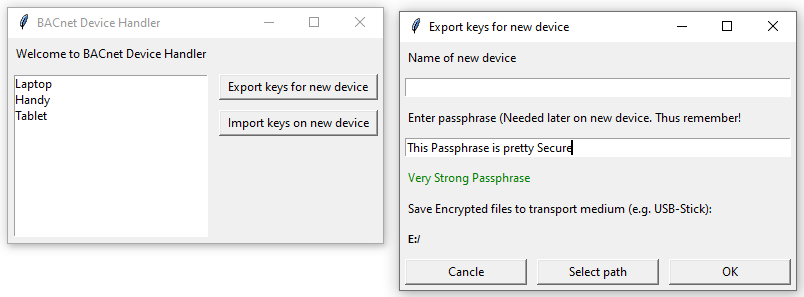
\includegraphics[width=1\textwidth]{figures/UI}
			\caption*{Das Hauptfenster und der geöffnete Exportdialog, welcher unter anderem die Passwortstärke angibt.}
		\end{figure}
		
		\subsubsection{}
		
\end{document}

